\documentclass[10pt,a4paper]{article}

\usepackage[utf8]{inputenc}		% Configuro la codificación
\input{.command.tex}
% En el siguiente archivo se configuran las variables del trabajo práctico
%% \providecommand es similar a \newcommnad, salvo que el primero ante un 
%% conflicto en la compilación, es ignorado.

% Al comienzo de un TP se debe modificar los argumentos de los comandos


\providecommand{\myTitle}{TRABAJO PRÁCTICO ESPECIAL}
\providecommand{\mySubtitle}{Análisis y procesamiento de la señal de habla}

\providecommand{\mySubject}{Señales y Sistemas (85.05)}
\providecommand{\myKeywords}{UBA, Ingeniería, 85.05, Señales y Sistemas}

% No es necesario modificar este
\providecommand{\myHeaderLogo}{header_fiuba}

\providecommand{\myAuthorSurname}{Manso}
\providecommand{\myTimePeriod}{Año 2016 - 2\textsuperscript{do} Cuatrimestre}


% Crear los integrantes del TP con el comando \PutMember donde
%%		1) Apellido, Nombre
%%		2) Número de Padrón
%%		3) E-Mail (Si el mail contiene '_', escribirlos como '\_'
\providecommand{\CoverMembers}[0]{
		\PutMember{Manso, Juan} {96133} {juanmanso@gmail.com}
}

\providecommand{\myLstLanguage}{Octave}

\Pagebreakfalse		% Setea si hay un salto de página en la carátula
\Indexfalse
\Siunitxfalse		% Si quiero utilizar el paquete, \siunixtrue. Si no \siunitxfalse
\Listingstrue		% Idem con paquete listings (programación)
\Keywordsfalse
				% Archivo con los comandos globales como Título y autores
%Preambulo para articulo científico de LaTeX

\usepackage[a4paper,left=3cm,right=3cm,bottom=3.5cm,top=3.5cm]{geometry} 	% Configuro la geometría del papel
%\usepackage{microtype}														% Mejora el "spacing" de las palabras
\usepackage[spanish]{babel} 												% Compatibilizo los signos del español
	\addto\captionsspanish{\renewcommand{\tablename}{Tabla}}				%% Redefino nombres preestablecidos por Babel
	\addto\captionsspanish{\renewcommand{\listtablename}{Índice de tablas}}	%% y así en vez de Cuadro dirá Tabla.
\usepackage{amsmath, amsfonts, amssymb}										% Entornos matemáticos, fuentes y símbolos
\usepackage{graphicx}														% Necesario para insertar figuras
\usepackage{fancyhdr}														% Para manipular headers y footers
\usepackage[usenames]{color}											% \color{color deseado} {lo que querés que tenga color}
\usepackage{subcaption}														% Permite captions del tipo 1a, 1b
\usepackage{multirow}														% Para tablas
\usepackage{float}

\ifListings
	\usepackage{listingsutf8}

	\definecolor{mygreen}{rgb}{0,0.6,0}
	\definecolor{mygray}{rgb}{0.5,0.5,0.5}
	\definecolor{mymauve}{rgb}{0.58,0,0.82}
	
	\providecommand{\lstinputpath}[1]{\lstset{inputpath=#1}}

	\lstset{
		backgroundcolor=\color{white},   % choose the background color; you must add \usepackage{color} or \usepackage{xcolor}
		inputencoding=utf8/latin1,
		basicstyle=\ttfamily\footnotesize,        % the size of the fonts that are used for the code
		breakatwhitespace=false,         % sets if automatic breaks should only happen at whitespace
		breaklines=true,                 %% sets automatic line breaking
		captionpos=t,                    %% sets the caption-position to top 
		commentstyle=\color{mygreen},    % comment style
		deletekeywords={...},            % if you want to delete keywords from the given language
		escapeinside={\%*}{*)},          % if you want to add LaTeX within your code
		extendedchars=true,              % lets you use non-ASCII characters; for 8-bits encodings only, does not work with UTF-8
		frame=single,	                 %% adds a frame around the code
		keepspaces=true,                 % keeps spaces in text, useful for keeping indentation of code (possibly needs columns=flexible)
		keywordstyle=\color{blue},       % keyword style
		language=C++,		 	 %% the language of the code
		otherkeywords={*,...},           % if you want to add more keywords to the set
		numbers=left,                    %% where to put the line-numbers; possible values are (none, left, right)
		numbersep=5pt,                   %% how far the line-numbers are from the code
		numberstyle=\tiny\color{mygray}, % the style that is used for the line-numbers
		rulecolor=\color{black},         % if not set, the frame-color may be changed on line-breaks within not-black text (e.g. comments (green here))
		showspaces=false,                % show spaces everywhere adding particular underscores; it overrides 'showstringspaces'
		showstringspaces=false,          % underline spaces within strings only
		showtabs=false,                  % show tabs within strings adding particular underscores
		stepnumber=1,                    % the step between two line-numbers. If it's 1, each line will be numbered
		stringstyle=\color{mymauve},     % string literal style
		tabsize=4,	                   % sets default tabsize to 2 space
		title={\protect\filename@parse{\lstname}\protect\filename@base\text{.}\protect\filename@ext}	 %% show the filename of files included with \lstinputlisting; also try caption instead of title
	}
	 \usepackage{algpseudocode}						% Para pseudocodigo
	 \renewcommand{\algorithmicwhile}{\textbf{mientras}} 
	 \renewcommand{\algorithmicdo}{\textbf{hacer}} 
	 \renewcommand{\algorithmicfor}{\textbf{para}}
	 \renewcommand{\algorithmicreturn}{\textbf{devolver}}
	 \renewcommand{\algorithmicend}{\textbf{fin}} 
	 
	 \newcommand{\rpm}{\raisebox{.2ex}{$\scriptstyle\pm$}}  
\fi

\ifSiunitx
\usepackage{siunitx}											% Unidades: \SI {cantidad} {\unidad} (necesita texlive-science)
	\sisetup{load-configurations = abbreviations}							% Habilita poner \cm en vez de \centi\metre
	\sisetup{output-decimal-marker = {,}}									% Cambia los puntos decimales por comas
\fi

\usepackage{booktabs}														% Permite hacer tablas sin separadores en el medio
\usepackage{placeins}														
		\let\Oldsection\section												%% Permite que los flotantes (como figuras) no aparescan
	\renewcommand{\section}{\FloatBarrier\Oldsection}						%% antes o después de su sección correspondiente.
		\let\Oldsubsection\subsection
	\renewcommand{\subsection}{\FloatBarrier\Oldsubsection}		
		\let\Oldsubsubsection\subsubsection
	\renewcommand{\subsubsection}{\FloatBarrier\Oldsubsubsection}
\usepackage{hyperref}														% Debe ser agregado al final del preambulo

\hypersetup
{    bookmarks=true,         % show bookmarks bar?
     unicode=false,          % non-Latin characters in Acrobat’s bookmarks
     pdftoolbar=true,        % show Acrobat’s toolbar?
     pdfmenubar=true,        % show Acrobat’s menu?
     pdffitwindow=false,     % window fit to page when opened
     pdftitle={\myTitle},    		 % title
     pdfauthor={\myAuthorSurname},   % author
	 pdfcreator={\myAuthorSurname},	 % creator = author
     pdfsubject={\mySubject},		 % subject of the document
     pdfkeywords={\myKeywords},
     colorlinks=true,        % false: boxed links; true: colored links
     linkcolor=black,        % color of internal links (change box color with linkbordercolor)
     citecolor=black,        % color of links to bibliography
     filecolor=magenta,      % color of file links
     urlcolor=cyan           % color of external links
}

%Configuro la pagina con los encabezaos y pies de paginas
\pagestyle{fancy}										% Para agregar encabezados y pie de paginas	
\lhead{\mySubject}										% Encabezado izquierdo
\rhead{\includegraphics[scale=0.15]{\myHeaderLogo}} 	% Encabezado derecho (logo de la FIUBA)					


% Defino el path de los includegraphics
\graphicspath{{./Figuras/}}		% Directorio que contiene los graficos

% Defino el path para los input de .tex y de .eps
\makeatletter
\def\input@path{{./Figuras/}{./Secciones/}{./Cover_page/}}
\makeatother

% Defino el path del listings
\ifListings
%% Cambiar el nombre de la carpeta si se utilizan Listings
	\lstinputpath{../Secciones}
\fi

\providecommand{\graficarPNG}[4]{
			\begin{figure}[h!]
				\centering
					\includegraphics[scale=#1]{#2}
					\caption{#3}
					\label{#4}
			\end{figure}

}



\begin{document}
		% Carátula (formal o simple,_formal o _simple respectivamente),
		% Resumen e Índice (si es necesario configurar en config.tex) del informe
		\begin{titlepage}
	
		\thispagestyle{empty}

		\begin{center}
			
\includegraphics[scale=1.3]{Logo_Fiuba2}\\
			\large{\textsc{Universidad de Buenos Aires}}\\
			\large{\textsc{Facultad De Ingeniería}}\\
			\small{\myTimePeriod}
		\end{center}

		\vfill

		\begin{center}
			\Large{\underline{\textsc{\mySubject}}}
		\end{center}

		\vfill

		\begin{tabbing}
			\hspace{2cm}\=\+\myTitle\\
				TEMA: \mySubtitle\\
				FECHA: \today\\
			\\
				\MembersHeader
				\MembersOnCover	
		\end{tabbing}

%		\begin{abstract}
%			% Ejemplo de Resumens
%% MANTENER EL NOMBRE %%
	El siguiente trabajo práctico tiene como objetivo hacer uso de técnicas y herramientas de análisis de señales y sistemas, aplicándolas al análisis y procesamiento de la señal de habla.



%		\end{abstract}

	\ifKeywords
		\begin{center}
			\emph{Palabras Clave: \myKeywords}
		\end{center}
	\fi	

		\vfill
	
\end{titlepage}

\ifPagebreak
	\thispagestyle{empty}
	\ifIndex
		\tableofcontents
%		\listoffigures
%		\listoftables
	\fi

	\pagebreak
\fi



	\setcounter{page}{1}

	
\section{Ejercicio 1} \label{sec:ej1}
	\begin{flushleft}
		\textit{Analizar el fragmento musical que contiene el archivo} \texttt{audio.wav} \textit{mediante el
espectrograma de banda ancha y banda angosta. Describir qué es lo que se puede observar en
ambos casos y explicar el criterio usado para la elección de los parámetros.}
	\end{flushleft}

	\subsection{Consideraciones previas}
		En este Ejercicio se requieren los espectrograma de banda ancha (buena definición en frecuencia) y de banda angosta (buena definición en tiempo). Al aumentar la resolución en tiempo, baja necesariamente la resolución en frecuencia y viceversa. Por lo tanto el espectrograma de banda ancha carecerá de buena definición de las frecuencias en tiempo y en el de banda angosta sucederá lo mismo con la frecuencias entre sí.

		En orden de definir un ancho de ventana correcto, se requiere una relación entre las muestras y el tiempo que representan.

			\begin{equation}
				n = t \cdot F_S
			\end{equation}
			\label{eq:ntFs}

		Dado que el conversor analógico-digital toma una señal de tiempo total $t$ y se la muestrea con frecuencia de muestreo $F_S$, la señal discreta tendrá $n$ elementos. A partir de esto, se obtiene la ecuación \eqref{eq:ntFs}. En particular, la señal del archivo \texttt{audio.wav} fue muestreada con $F_S=\SI{16}{\kHz}$.


	\subsection{Banda ancha}
		Para una buena resolución en frecuencia, las ventanas del espectrograma deben ser grandes. Considerando que $\Delta f=\SI{0.5}{\Hz}$ es un intervalo apropiado de frecuencia, se desprende el siguiente cálculo (a partir de \eqref{eq:ntFs}).

		\begin{align*}
			l_{ventana} &= t_{ventana} \cdot F_S\\
			l_{ventana} &= \frac{1}{\Delta f} \cdot F_S\\
			l_{ventana} &= \frac{\SI{16}{\kHz}}{\SI{0.5}{\Hz}}\\
			\Rightarrow l_{ventana} &= 2 \cdot F_S = \num{32000}\\
		\end{align*}

		Se define además un \textit{overlap} de un tercio del largo de la ventana (para tener suavidad en la curva) y la ventana del tipo \textit{Hamming}. Así se obtiene el espectrograma de la Figura \ref{graf:banda_ancha}.

	\begin{figure}
		\centering
		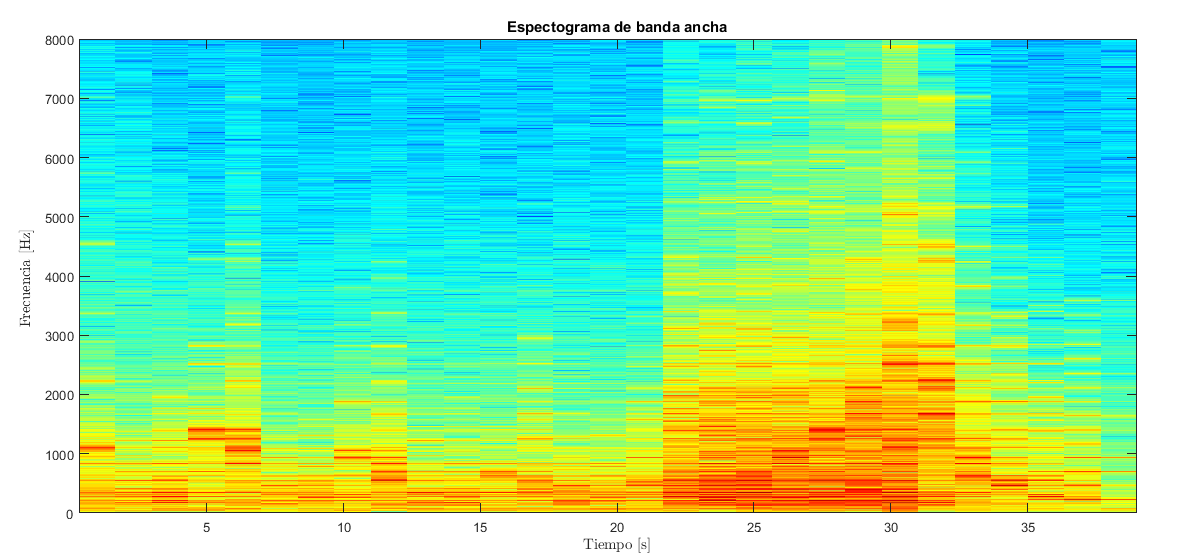
\includegraphics[scale=0.35]{1a.png}
		\caption{Espectrograma de banda ancha.}
		\label{graf:banda_ancha}
	\end{figure}

	\subsection{Banda angosta}
	
		\begin{figure}[h!]
			\centering
			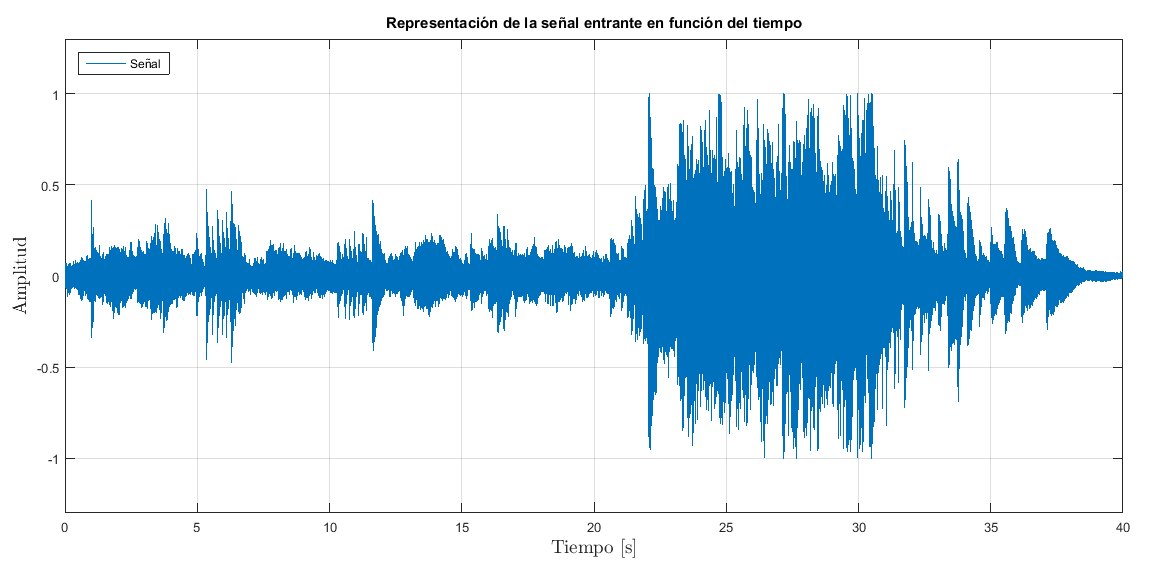
\includegraphics[scale=0.35]{Senal_temporal.png}
			\caption{Señal del archivo \texttt{audio.wav}.}
			\label{graf:senal_original}
		\end{figure}


		Suponiendo que la señal fuese un tren de pulsos, un criterio válido sería que haya 10 ventanas por pulso. A partir del gráfico de la señal de la Figura \ref{graf:senal_original}, se escoge como pulso patrón el representado en la Figura \ref{graf:pulso_patron}.

		\begin{figure}[h!]
			\centering
			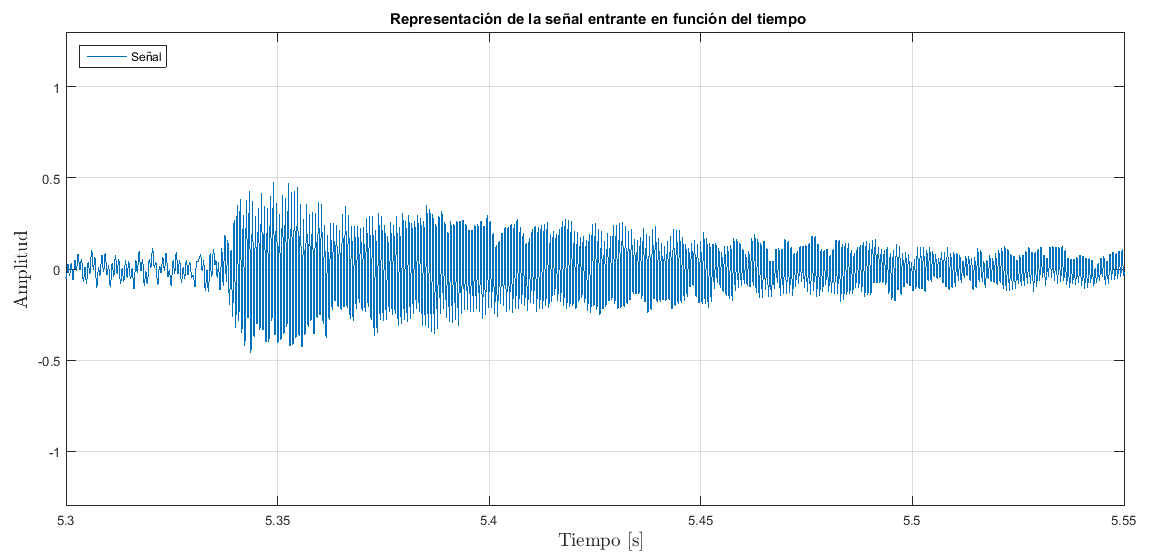
\includegraphics[scale=0.35]{Pulso_temporal.png}
			\caption{Parte de la señal original que se utiliza como patrón.}
			\label{graf:pulso_patron}
		\end{figure}

		Por lo tanto, como $t_{ventana}=\SI{.2}{\s}$:
			\begin{align*}
				10\cdot l_{ventana} &= t_{ventana} \cdot F_S\\
				l_{ventana} &= \frac{\SI{0.2}{\s} \cdot \SI{16}{\kHz}}{10}\\
				\Rightarrow l_{ventana} &= \frac{F_S}{50} = 320\\
			\end{align*}

		Con el mismo \textit{overlap} relativo y utilizando ventanas de \textit{Hamming} se obtiene el espectrograma de la Figura \ref{graf:banda_angosta}.

		\begin{figure}[h!]
			\centering
			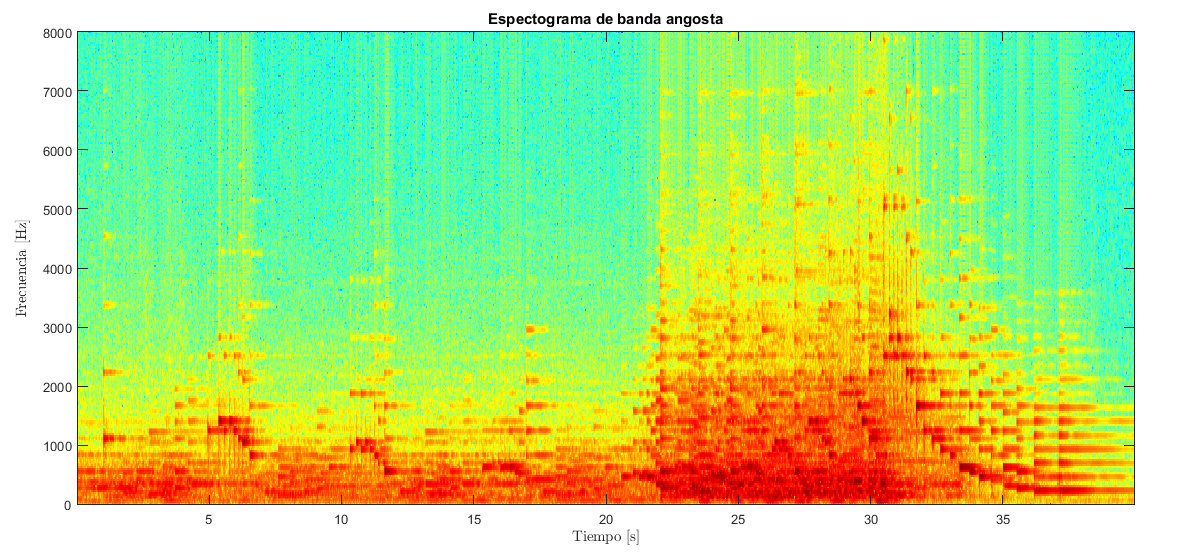
\includegraphics[scale=0.35]{1b.png}
			\caption{Espectrograma de banda angosta.}
			\label{graf:banda_angosta}
		\end{figure}

	

\section{Ejercicio 2}
	\begin{flushleft}
		\textit{Usando la información obtenida en el ejercicio anterior, obtener los parámetros del
espectrograma que permitan observar de la mejor manera posible las características tiempo-
frecuencia de este archivo de audio. Por medio de este espectrograma debe ser posible
identificar las siguientes notas del piano cuyas frecuencias aproximadas se representan en la Tabla \ref{tab:notas}.}
	\end{flushleft}

	\begin{table}[H]
		\centering
		\begin{tabular}{*{12}{c}}
			\toprule
			Do&Do\# &Re&Re\# &Mi&Fa&Fa\# &Sol&Sol\# &La&La\# &Si\\
			\midrule
			523&554&587&622&659&698&740&784&831&880&932&988\\
			1046&1108&1174&1244&1318&1386&1480&1568&1662&1760&1864&1976\\
			\bottomrule
		\end{tabular}
		\caption{Frecuencias que representan las notas musicales en su cuarta y quinta octava.}
		\label{tab:notas}
	\end{table}

	\subsection{Parámetros del espectrograma}
		De la Tabla \ref{tab:notas} se ve que el intervalo más corto de frecuencias es $554-523=31=\Delta f_{\min}$. Además por el Ejercicio \ref{sec:ej1}, se sabe que $\Delta t_{\min}=\SI{0.2}{\s}$. Por lo tanto:
		\begin{align*}
			F_S \cdot \SI{0.2}{\s} = \frac{F_S}{\SI{5}{\Hz}} > l_{ventana} &> \frac{F_S}{\SI{31}{\Hz}}\\
		\end{align*}

		Se propone utilizar $l_{ventana}=\frac{F_S}{\SI{10}{\Hz}}$ y resulta el gráfico de la Figura \ref{graf:spec_ej2}.
		Como criterio se propone un error relativo del 10\%. Si el error es menor, la representación se considerará correcta.

		\begin{figure}[h!]
			\centering
			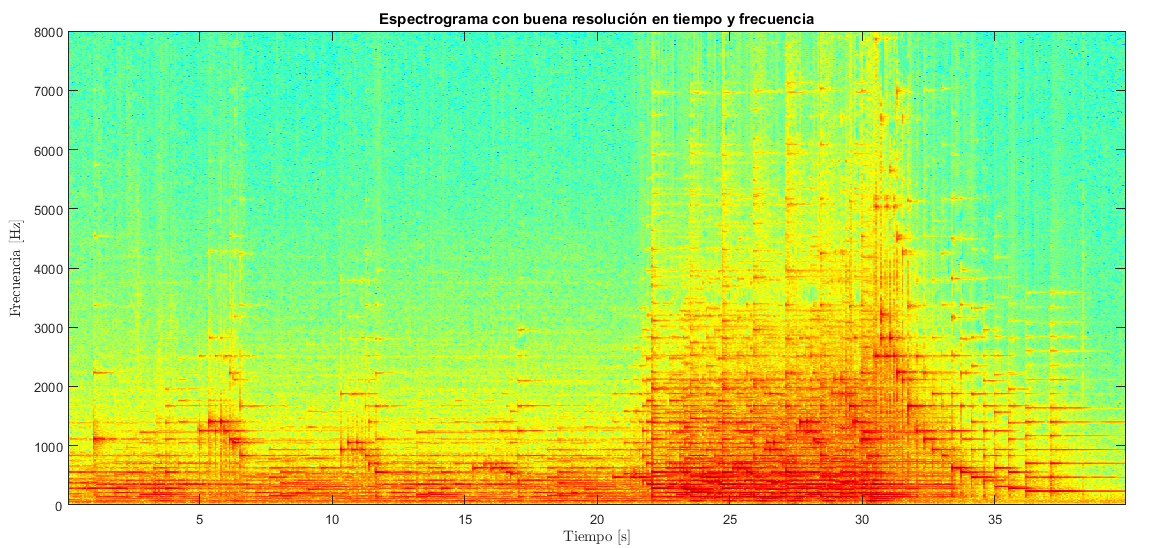
\includegraphics[scale=0.35]{2.png}
			\caption{Espectrograma de precisión.}
			\label{graf:spec_ej2}
		\end{figure}

	\subsection{Detección de las notas}
		Se buscaron las frecuencias que representan a las notas musicales en el espectograma y se obtuvieron sus valores más próximos expuestos en la Tabla \ref{tab:comparativa1} y sus respectivos errores en la Tabla \ref{tab:comparativa2}.

	\begin{table}[H]
		\centering
		\begin{tabular}{*{12}{c}}
			\toprule
			Do&Do\# &Re&Re\# &Mi&Fa&Fa\# &Sol&Sol\# &La&La\# &Si\\
			\midrule
			\num{523.44}&\num{554.69}&\num{585.94}&\num{625}&\num{656.25}&\num{695.31}&\num{742.19}&\num{781.25}&\num{828.13}&\num{882.81}&\num{929.69}&\num{992.19}\\
			\num{1046.9}&\num{1109.4}&\num{1171.9}&\num{1242.2}&\num{1320.3}&\num{1390.6}&\num{1484.4}&\num{1570.3}&\num{1664.1}&\num{1765.6}&\num{1867.2}&\num{1976.6}\\
			\bottomrule
		\end{tabular}
		\caption{Frecuencias del espectrograma más próximas a las de la tabla \ref{tab:notas}.}
		\label{tab:comparativa1}
	\end{table}

	\begin{table}[H]
		\centering
		\begin{tabular}{*{12}{c}}
			\toprule
			Do&Do\# &Re&Re\# &Mi&Fa&Fa\# &Sol&Sol\# &La&La\# &Si\\
			\midrule
			\num{0.4375}&\num{0.6875}&\num{1.0625}&\num{3}&\num{2.75}&\num{2.6875}&\num{2.1875}&\num{2.75}&\num{2.875}&\num{2.8125}&\num{2.3125}&\num{4.1875}\\
			\num{0.875}&\num{1.375}&\num{2.125}&\num{1.8125}&\num{2.3125}&\num{4.625}&\num{4.375}&\num{2.3125}&\num{2.0625}&\num{5.625}&\num{3.1875}&\num{0.5625}\\
			\bottomrule
		\end{tabular}
		\caption{Diferencia entre las frecuencias del espectrograma que representan a las notas y las reales.}
		\label{tab:comparativa2}
	\end{table}

	A partir de estas tablas se ve que la máxima diferencia es de \num{5.625} (5\textsuperscript{ta} octava del La) y el error relativo máximo es de 0,5\% (4\textsuperscript{ta} octava de Re). Al estar dentro del criterio propuesto, el espectograma permite identificar las notas requeridas.


	

\section{Ejercicio 3} \label{ej3}
	\begin{flushleft}
		\textit{Se pretende duplicar la duración del fragmento musical para lo cual se propone interpolar el
archivo de audio. No está permitido usar las funciones de matlab/octave que implementan la
interpolación directamente. Grafique el espectrograma de la nueva secuencia y compárela con
la obtenida en el Ejercicio 2.}
	\end{flushleft}

	\subsection{Interpolación}
		El algoritmo de interpolación lineal se simplifica al contar con el álgebra matricial propio del \textit{Matlab}. La rutina se resume a continuación:
		\begin{lstlisting}
	doble_audio = linspace(0,1,length(audio)*2);
	doble_audio(1:2:end) = audio;
	doble_audio(2:2:end-1)=(audio(2:end)-audio(1:end-1))/2+audio(1:end-1);
		\end{lstlisting}

	\subsection{Comparación de espectogramas}

		\begin{figure}[h!]
			\centering
			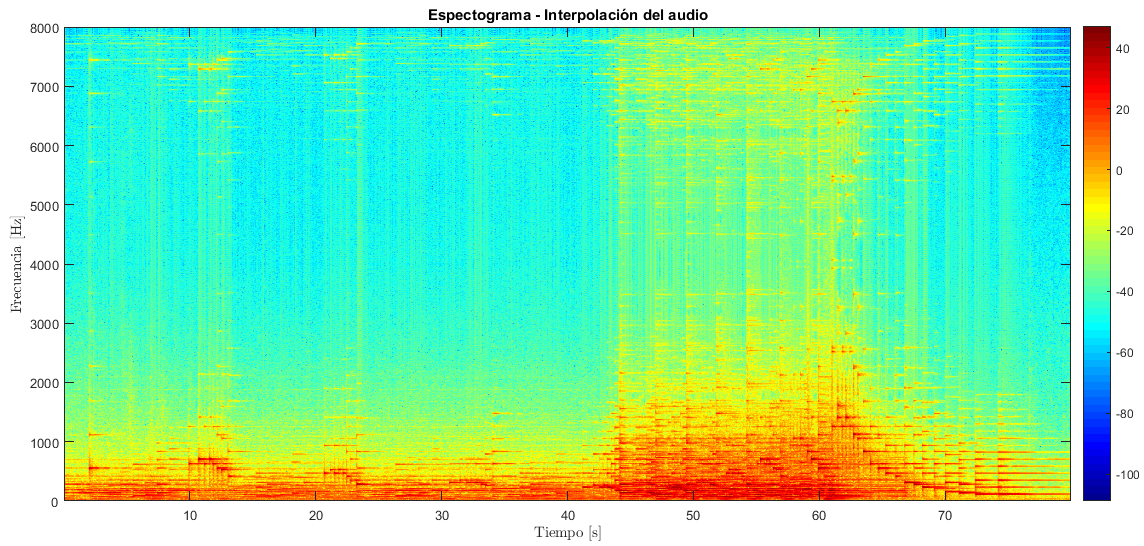
\includegraphics[scale=0.35]{3.png}
			\caption{Espectrograma de la señal interpolada.}
			\label{graf:ej3}
		\end{figure}
		Al interpolar la señal original, se obtiene el doble de muestras. Ante una misma $F_S$ (Figura \ref{graf:ej3}), la duración de la señal interpolada será el doble. A su vez, el espectro de frecuencias se comprime en 2.\\

		\graficarPNG{0.35}{3bis}{Espectrograma de la señal interpolada con $F_S^*=2 F_S$.}{graf:ej3bis}
		Realizando el espectograma de la señal interpolada con $F_S^*=2F_S$ (Figura \ref{graf:ej3bis}), se ve que las frecuencias son las mismas. Por lo tanto, si se reconstruyen ambas señales con sus respectivas frecuencias de muestreo se obtiene la misma señal.

		Por otro lado se ve que, debido a la interpolación, se presentan componentes de alta frecuencia que la original carecía ($f>\SI{8}{\kHz}$ con $F_S^*=2F_S$). Esto se debe a que, al ser periodica la DFT, la compresión del espectro copia parte del mismo espectro espejado. Por lo tanto, se propone realizar un filtrado pasabajos. El filtro a utilizar es una ventana rectangular en frecuencia. En la Figura \ref{graf:ej3bis_b} se expone el espectrograma de la señal interpolada y filtrada posteriormente.

		\graficarPNG{0.35}{3bbis}{Espectrograma de la señal interpolada filtrada con $F_S^*=2 F_S$.}{graf:ej3bis_b}

		Se podría interpretar que al aplicar el filtro la señal presentaría más ruido (zonas previamente en azul se grafican amarillas ahora). Esto se debe a que el graficador toma el valor más pequeño y lo define como azul oscuro. Se puede ver en las Figuras \ref{graf:ej3_comp} y \ref{graf:ej3_comp_b} que un mismo punto mantiene el valor de $z$ (denominada \textit{Index} en los gráficos). Por lo tanto, la señal filtrada es más fiel a la original dado que carece de los componentes de alta frecuencia parásitos.

		\graficarPNG{0.35}{3_comp}{Espectrograma para comparar - Interpolación sin filtro.}{graf:ej3_comp}
		\graficarPNG{0.35}{3b_comp}{Espectrograma para comparar - Interpolación con filtro.}{graf:ej3_comp_b}

	

\section{Ejercicio 4}	\label{ej4}
	\begin{flushleft}
	\textit{Reducir a la mitad la duración del fragmento musical utilizando el proceso de decimación.
No está permitido usar las funciones de matlab/octave que implementan la decimación
directamente. Recuerde que para evitar el aliasing es necesario realizar el adecuado filtrado
pasabajos. Utilice alguno de los métodos de diseño explicados en la teórica especificando el
criterio utilizado. Grafique el espectrograma de la nueva secuencia y compárela con la obtenida
en el Ejercicio 2.}
	\end{flushleft}

	\subsection{Decimación}
	Se recuerda que, cuando se decima por N una señal discreta que fue muestreada, al comprimir el espectro de frecuencias, la señal útil queda entre $-\pi/N$ y $\pi/N$ (en vez de $-\pi$,$\pi$). Todo lo demás tendrá aliasing al pasar por el conversor digital analógico (DAC). Por ende, como se pretende decimar por $N=2$, se aplica un pasabajos ideal entre $-\pi/2$ y $\pi/2$ (o en frecuencia $-F_S/4$, $F_S/4$). Dado que la función \texttt{fft()} da los valores entre 0 y $2\pi$, sólo se requiere eliminar desde $\pi/2$ hasta $\frac{3}{2}\pi$. Se utiliza el parámetro \texttt{'symmetric'} de la función \texttt{ifft()} para que sea posible reconstruir al poner ceros desde $\pi/2$ hasta $2\pi$ en el espectro de frecuencias.

		A continuación se expone la implementación utilizada:
		\begin{lstlisting}
aux=audio;

% Pasaje a frecuencia
NFFT=2^nextpow2(length(aux));
fft_mitad=fft(aux,NFFT);

% Frecuencias menores y mayores a |Fs/4| ==> =0
fft_mitad(fix(length(fft_mitad)/4)+1:end)=0;

% Reconstruccion
% Como se elimino desde 3/2*pi hasta 2*pi, queda asimetrica, por lo tanto
% se utiliza el parametro 'symmetric' para solucionarlo.
aux=ifft((fft_mitad),'symmetric');

% Decimacion.
mitad_audio=aux(1:2:end-1);
mitad_audio=mitad_audio(1:round(length(audio_input)/2));
		\end{lstlisting}


	\subsection{Comparación de espectrogramas}

	Como se sabe, al comprimir el dominio del tiempo, se expande el dominio de las frecuencias. Así, se ve en la Figura \ref{graf:ej4} compensando la frecuencia de muestreo, el eje de frecuencias se expande en 2 con respecto a la original (Figura \ref{graf:spec_ej2}).

		\graficarPNG{0.35}{4bis}{Espectrograma de la señal decimada con frecuencia de muestreo compensada.}{graf:ej4}

	
\pagebreak
\section{Ejercicio 5} \label{ej5}
	\begin{flushleft}
		\textit{Desarrolle un programa que a partir del espectrograma de la señal de audio permita
reconstruir la señal original. Grafique el error entre la señal original y la reconstruida.}
	\end{flushleft}

	\subsection{Implementación final}	
	\lstinputlisting{../../rec_spec.m}

	\subsection{Comparación}

		\graficarPNG{0.35}{5a}{Espectrograma de la señal reconstruida sin compensación de ventanas.}{graf:rec_a}

		De la Figura \ref{graf:rec_a}, se ve que las frecuencias de la reconstruida carecen de la definición de la original. En particular, en la zona de frecuecias medias, la reconstruida presenta más naranja que su contraparte que contiene sectores más azules y rojas (mayor exactitud).\\

		La razón de esta diferencia es la utilización de ventanas. El proceso de seccionar una porción de la señal es equivalente a multiplicarla por un pulso de longitud finita. Por Fourier se sabe que la multiplicación de dos señales en tiempo, resulta en una convolución de sus transformadas en frecuencia. Así, de utilizar un pulso rectangular por ejemplo, se haría la convolución con una curva que no es una delta, alterando la señal (en el ejemplo, una función \textit{sinc}). Por lo tanto, al reconstruirla a partir de su transformada, la señal presenta impresición en el dominio de las frecuencias debido al ventaneo previo.\\

		En particular, tomando como punto de comparación al tiempo \SI{30}{\s}, para las frecuencias de \SI{380}{\Hz} y \SI{1100}{\Hz} la diferencia es de aproximadamente 30\% como se ve en la Figura \ref{graf:dft_5b}.\\

		\graficarPNG{0.35}{5-dft2}{DFT de las señales orginial y reconstruida a tiempo $t=\SI{30}{\s}$}{graf:dft_5b}

		Al utilizar la ventana de \textit{Hamming}, se minimiza el lóbulo más próximo al fundamental, siendo éste muy angosto. Del mismo modo que con la ventana rectangular, la señal debe ser compensada del efecto de la ventana. Por lo tanto, en las líneas 18 y 26 del código de la función, se divide la ventana a concatenar por los coeficientes de la ventana de \textit{Hamming}. Este cambio logra una reconstrucción completa de la señal original. A continuación se presenta el espectrograma de la implementación final:\\

		\graficarPNG{0.35}{5b}{Espectrograma de la señal reconstruida con compensación de ventanas.}{graf:rec}

		Como se puede ver en la Figura \ref{graf:rec}, la reconstrucción mejora. En particular, al hacer la misma comparación en $t=\SI{30}{\s}$ (Figura \ref{graf:dft_5}) se comprueba que la reconstrucción es precisa.

		\graficarPNG{0.35}{5-dft}{DFT de las señales orginial y reconstruida compensada a tiempo $t=\SI{30}{\s}$}{graf:dft_5}

	

\section{Ejercicio 6} \label{ej6}
	\begin{flushleft}
		\textit{Suponiendo que utilicen la función} specgram\textit{, cada columna contiene información del
espectro para ese segmento de la señal. Con el objeto de duplicar la duración de la secuencia
original interpole una columna cada dos utilizando la información de las filas. Luego utilizando
el programa desarrollado en el punto anterior encuentre la nueva señal de audio que debería
durar el doble de tiempo. Grafique su espectrograma y compárelo con el original.}
	\end{flushleft}

	\subsection{Implementación}

		Para la interpolación, se utilizaron los mismos pasos del Ejercicio \ref{ej3} con la excepción de que se interpola la matriz resultante del \texttt{specgram()}. Luego, se reconstruye con la función \texttt{rec\_spec()} del Ejercicio \ref{ej5}.

		\pagebreak
	\subsection{Comparación de espectrogramas y modificación de la implementación}

	\graficarPNG{0.35}{6}{Espectrograma de la señal resultante de la interpolación de las columnas de S.}{graf:ej6}

	Como se ve en la Figura \ref{graf:ej6}, la interpolación de las columnas del espectrograma no altera las frecuencias de la señal. Este resultado tiene sentido, dado que al interpolar la señal con sus componentes en frecuencia determinadas, dichas frecuencias se mantienen constantes logrando que la señal original duplique su longitud. Al igual que en el Ejercicio \ref{ej3}, la diferencia de colores se debe a la escala que utiliza el \texttt{specgram()} para graficar.\\

	\graficarPNG{0.35}{6ns}{Discontinuidad de la señal al expandir las columnas del espectograma y volver a tiempo.}{graf:ej6_no_suave}
	Sin embargo, al escuchar dicho audio se encuentran ruidos impropios de la señal original. Haciendo énfasis en la señal temporal, se ve que la unión de las ventanas no es suave (Figura \ref{graf:ej6_no_suave}). La razón de este comportamiento indeseado es la interpolación de las columnas. Las nuevas columnas se transforman en tiempo como ventanas nuevas cuyos puntos iniciales y finales pueden diferir de los que se concatenarán después.\\

	Es por eso que se propone expandir las columnas con la columna previa. Así se duplicaría el largo del audio concatenando ventanas con si mismas (y luego la última concatenaría suavemente con la siguiente ventana). Ésto mejora auditivamente la señal, dando un efecto de duración más evidente en vez del eco generado por la primer implementación. A pesar de esto, la curva sigue siendo discontinua persistiendo el ruido.\\

	Se propone por lo tanto pedir que la unión sea continua y que la derivada de la misma también lo sea. Dicha implementación se presenta a continuación con su gráfico en la Figura \ref{graf:ej6_suave}:

	\begin{lstlisting}
for x=1:(rows-1)
	concat=aux(x+1,noverlap+1:end)./window(noverlap+1:end);

	for y=1:(length(concat)-1)
		checkeo1=(concat(y)-output(end))/output(end);

		if(-0.1<=checkeo1 && checkeo1<=0.1)
			checkeo2=(concat(y+1)-concat(y))/(output(end)-output(end-1));

			if(0.9<=checkeo2 && checkeo2<=1.1)
				concat=[concat(y:end)];
				break;
			end
		end
	end
	output=[output concat];
end
	\end{lstlisting}

	\graficarPNG{0.35}{6s}{Mejora en la discontinuidad de la reconstrucción de la señal.}{graf:ej6_suave}

	Como se puede ver en la Figura \ref{graf:ej6_suave}, la continuidad de la señal mejora considerablemente. Analizando diferentes uniones de ventanas de la señal (para comprobar la generalidad del método) se encontraron problemas como el de la Figura \ref{graf:ej6_suave_problema}. En dicho gráfico se ve que la señal tiene cierta suavidad en la unión, pero la senoide envolvente cambia de signo su pendiente. Dado que el método es básico, no se pretende obtener una señal perfecta, por lo tanto se pasa por alto este error.
	\graficarPNG{0.35}{6sprob}{Problema al concatenar ventanas.}{graf:ej6_suave_problema}

	Al utilizar el algoritmo descripto por el espectograma de \texttt{audio.wav}, mejora considerablemente la calidad del nuevo audio. Sin embargo, por los problemas de suavidad y cambio de pendientes, se encuentran momentos más ruidosos que otros. Puede deberse también a que el error en ciertas zonas es imperceptible para un oido no entrenado y en otros lo es. De todos modos, la nueva implementación mejora considerablemente al audio.

	

\section{Ejercicio 7} \label{ej7}
	\begin{flushleft}
		\textit{Ahora se busca reducir la duración del audio a la mitad para lo cual se debe decimar el
espectrograma por columnas. Recuerde que para evitar el aliasing es necesario realizar el
adecuado filtrado pasabajos.}
	\end{flushleft}

	\subsection{Implementación}

	Para resolver este ejercicio, se realizó la misma rutina que la del Ejercicio \ref{ej4}	pero, al contar con los coeficientes de la transformada en el vector del \texttt{specgram()} no se requiere el pasaje a frecuencia ni el filtrado de dicho ejercicio (por la misma razón del ejercicio \ref{ej6}). Después de ello, se reconstruye con la función del Ejercicio \ref{ej5}.

	\subsection{Comparación de espectrogramas}


	\graficarPNG{0.35}{7}{Espectrograma de la señal resultante de la decimación de las columnas de S.}{graf:ej7}

	Al igual que en el Ejercicio \ref{ej6}, el espectograma es similar al del Ejercicio \ref{ej5} exceptuando la longitud del mismo. Utilizando la nueva implementación que suaviza las uniones, el audio contiene los mismos problemas que el Ejercicio anterior.\\

	Merece ser mencionado que no se realizó un filtrado pasabajos de la señal, porque la interpolación es de muestras con \emph{dft} predeterminada previamente. Otra propuesta interesante sería interpretar a las filas del espectrograma como señales individuales. Así se podría realizar la \emph{dft} de dichas señales y aplicar el filtro \emph{antialiasing}. Dado que el dichas señales no fueron muestreadas por \emph{Nyquist} y su posible dependencia con las ventanas y overlap utilizados, aplicar dicho método puede resultar erroneo. Sin embargo es interesante el enfoque de analizar las variaciones de amplitud de una ventana de frecuencias como una señal temporal ordinaria.


	
\section{Conclusiones} 

	Del análisis y resolución de los Ejercicios \ref{ej3} y \ref{ej4} se puede concluir que los métodos de expansión o decimación de muestras no son efectivos para variar la duración de señales. La razón principal es que la variación en la duración genera una variación en el espectro de frecuencias. A pesar de ello, estos métodos son útiles para compresión o expansión del tamaño de los archivos de audio. Si se modifica la frecuencia de muestreo del DAC de modo que la duración y frecuencias sean similares a la original, lo que se obtiene es una variación en el tamaño del archivo. Así, si la señal inicial fue sobremuestreada (es decir el espectro de la misma es de banda mucho más angosta que $F_S$), una decimación y reconstrucción apropiada mantendría la calidad previa del audio haciendo que éste pese menos.\\

	Por el otro lado, el método propuesto por los Ejercicios \ref{ej6} y \ref{ej7} es más apropiado para variar la duración de la señal, manteniendo el espectro original. En estos casos, las diferencias numéricas son pequeñas pero auditivamente apreciables. Para mayor precisión haría falta recurrir a otros métodos como por ejemplo concatenar ventanas en el mismo valor y que éste sea 0 (método disponible en \emph{software} de edición de audio como \emph{Cubase} y \emph{Pro Tools}).


\end{document}
